\whiteBGstarBegin
\setcounter{section}{0}
\section{Trắc nghiệm}
\begin{enumerate}[label=\bfseries Câu \arabic*:]
	
	\item \mkstar{1}
	
	\cauhoi{ Muốn cho một chất điểm cân bằng thì hợp lực của các lực tác dụng lên nó phải	
		\begin{mcq}(2)
			\item không đổi.
			\item thay đổi.
			\item bằng 0.
			\item khác 0.
		\end{mcq}
	}
	
	\loigiai{
		\textbf{Đáp án: C.}
		
		Muốn cho một chất điểm cân bằng thì hợp lực của các lực tác dụng lên nó phải bằng 0.
	}
	\item \mkstar{1}
	
	\cauhoi{ Độ lớn của hợp lực $\vec{F}$ hai lực $\vec{F}_1$ và $\vec{F}_2$  đồng qui hợp với nhau góc $\alpha$ là
		\begin{mcq}(2)
			\item $\sqrt{F_1^2+F_2^2-2F_1F_2\cos \alpha}$.
			\item $\sqrt{F_1^2+F_2^2+2F_1F_2\cos \alpha}$.
			\item $\sqrt{F_1^2+F_2^2-F_1F_2\cos \alpha}$.
			\item $\sqrt{F_1^2+F_2^2+F_1F_2\cos \alpha}$.
		\end{mcq}
	}
	\loigiai{	
		\textbf{Đáp án: B.}
		
		Ta có: $$F = \sqrt{F_1^2+F_2^2+2F_1F_2\cos \alpha}.$$
	}
	\item \mkstar{1}
	
	\cauhoi{ Tổng hợp lực là 
		\begin{mcq}
			\item thay thế một lực bằng các lực có tác dụng giống hệt như các lực ấy.
			\item thay thế các lực tác dụng đồng thời vào cùng một vật bằng một lực có tác dụng giống hệt như các lực ấy.
			\item thay thế các lực tác dụng đồng thời hai vật bằng một lực có tác dụng giống hệt như các lực ấy.
			\item thay thế hai lực bằng ba lực có tác dụng giống hệt như các lực ấy.
		\end{mcq}
	}
	\loigiai{		\textbf{Đáp án: B.}
		
		Tổng hợp lực là thay thế các lực tác dụng đồng thời vào cùng một vật bằng một lực có tác dụng giống hệt như các lực ấy.
	}
	\item \mkstar{2}
	
	\cauhoi{ Một chất điểm đứng yên dưới tác dụng của $3$ lực có độ lớn bằng nhau. Kết luận nào sau đây là đúng?
		\begin{mcq}
			\item 	Có 2 lực cùng giá, ngược chiều nhau.
			\item  Ba lực có giá cùng nằm trong 1 mặt phẳng, chúng lần lượt hợp với nhau những góc $120^\circ$.
			\item Ba lực có giá cùng nằm trong một mặt phẳng, trong đó $2$ lực có giá vuông góc nhau.
			\item Cả A, B, C đều sai.
			
		\end{mcq}
	}
	\loigiai{		\textbf{Đáp án: B.}	
		
		Một chất điểm đứng yên dưới tác dụng của $3$ lực có độ lớn bằng nhau thì ba lực có giá cùng nằm trong 1 mặt phẳng, chúng lần lượt hợp với nhau những góc $120^\circ$.
	
	}
	\item \mkstar{2}
	
	\cauhoi{ Tác dụng vào một vật đồng thời hai lực $\vec{F_1}$  và $\vec{F_2}$ trong đó độ lớn $F_1 = 30\ \text{N}$ và $F_1 = 40\ \text{N}$. Nhận xét nào sau đây là đúng?
		\begin{mcq}
			\item Hợp lực tác dụng lên vật có độ lớn $70\ \text{N}$.
			\item Hợp lực tác dụng lên vật có độ lớn $10\ \text{N}$.
			\item Hợp lực tác dụng lên vật có độ lớn $50\ \text{N}$.
			\item Chưa đủ cơ sở để kết luận.
		\end{mcq}
	}
	\loigiai{		\textbf{Đáp án: D.}
		
		Vì chưa biết $\alpha$ hợp bởi hai lực  $\vec{F_1}$  và $\vec{F_2}$ nên ta chưa đủ cơ sở để kết luận.
	}


	\item \mkstar{2}
	
	\cauhoi{ Điều nào sau đây là \textbf{sai} khi nói về đặc điểm của hai lực cân bằng? 
		
		\begin{mcq}(2)
			\item Hai lực có cùng giá.
			\item Hai lực đặt vào hai vật khác nhau.
			\item Hai lực ngược chiều nhau.
			\item Hai lực có cùng độ lớn.
		\end{mcq}
	}
	\loigiai{		\textbf{Đáp án: B.}
		
		Hai lực cân bằng đặt vào cùng một vật.
		
	}

	\item \mkstar{2}
	
	\cauhoi{ Hai lực có giá đồng quy có độ lớn $F_1=F_2=10\ N$, có $(\overrightarrow {F_1}, \overrightarrow {F_2})=60^\circ$. Hợp lực của hai lực này có độ lớn là
		\begin{mcq}(4)
			\item $\text{17,3}\, \si{\newton}$.
			\item $\text{20}\, \si{\newton}$.
			\item $\text{14,1}\, \si{\newton}$.
			\item $\text{10}\, \si{\newton}$.
		\end{mcq}
		
	}
	\loigiai{		\textbf{Đáp án: A.}
		
		Áp dụng công thức $$F^2=F_1^2+F_2^2+2F_1F_2.\cos(\overrightarrow {F_1}, \overrightarrow {F_2}) $$
		
		Thay số liệu vào, ta tìm được $$F=\text{17,3}\, \si{\newton}$$
	}
	\item \mkstar{3}
	
	\cauhoi{ Một chất điểm chịu tác dụng đồng thời của hai lực thành phần có độ lớn $F_1$ và $F_2$ thì hợp lực F của chúng luôn có độ lớn thỏa mãn hệ thức:
		\begin{mcq}(2)
			\item $F=F_1^2+F_2^2$.
			\item $F = F_1 + F_2$.
			\item $|F_1-F_2| \leq F \leq F_1 + F_2$.
			\item $F= \sqrt{F_1^2+F_2^2}$.
		\end{mcq}
		
	}
	\loigiai{		\textbf{Đáp án: C.}
		
		Theo lý thuyết:	$$|F_1-F_2| \leq F \leq F_1 + F_2$$
		

	}
	\item \mkstar{3}
	
	\cauhoi{ Cho hai lực đồng quy có độ lớn bằng $12\ \text{N}$ và $16\ \text{N}$ hợp nhau một góc $\alpha$. Độ lớn và góc hợp bởi hai lực đó là 
		\begin{mcq}(2)
			\item $3\ \text{N}$ và $30^\circ$.
			\item $20\ \text{N}$ và $90^\circ$.
			\item $30\ \text{N}$ và $60^\circ$.
			\item $40\ \text{N}$ và $45^\circ$.
		\end{mcq}
	}
	\loigiai{		\textbf{Đáp án: B.}
		
		Với $\alpha=90^\circ$
		
		Độ lớn và góc hợp bởi hai lực đó là 
		$$F=\sqrt{F_1^2+F_2^2}=20\ \text{N}.$$
		

	}

	\item \mkstar{4}
	
	\cauhoi{ Một thanh đồng chất nằm cân bằng ở tư thế nằm ngang bởi hai sợi dây buộc vào hai đầu của nó như hình vẽ. Lực căng dây có độ lớn $T_1=T_2=\SI{10}{\newton}$, góc $\theta=37^\circ$. Trọng lượng của thanh bằng
		\begin{center}
			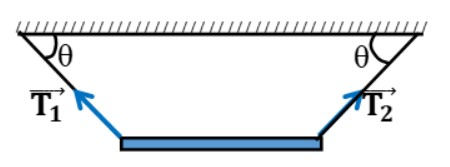
\includegraphics[scale=0.7]{../figs/VN10-2021-PH-TP011-5.jpg}
		\end{center}
		\begin{mcq}(4)
			\item $\SI{10}{\newton}$.
			\item $\SI{20}{\newton}$.
			\item $\SI{12}{\newton}$.
			\item $\SI{16}{\newton}$.
		\end{mcq}
		
		
	}
	\loigiai{		\textbf{Đáp án: C.}
		
		Trọng lượng của thanh bằng
		$$P=mg=2T\sin\theta=\SI{12}{\newton}.$$
		
	}
\end{enumerate}

\whiteBGstarEnd

\loigiai
{
	\begin{center}
		\textbf{BẢNG ĐÁP ÁN}
	\end{center}
	\begin{center}
		\begin{tabular}{|m{2.8em}|m{2.8em}|m{2.8em}|m{2.8em}|m{2.8em}|m{2.8em}|m{2.8em}|m{2.8em}|m{2.8em}|m{2.8em}|}
			\hline
			1.C  & 2.B  & 3.B  & 4.B  & 5.D  & 6.B  & 7.A  & 8.C  & 9.B  & 10.C  \\
			\hline
			
		\end{tabular}
	\end{center}
}
\section{Tự luận}
\begin{enumerate}[label=\bfseries Câu \arabic*:]
	\item \mkstar{1}
	
	\cauhoi{
	Phát biểu định nghĩa của lực và điều kiện cân bằng của một chất điểm.
	}
	
	\loigiai{
		
	Lực là một đại lượng vec-tơ đặc trưng cho sự tác dụng của vật này vào vật khác mà kết quả là gây ra gia tốc cho vật hoặc làm cho vật bị biến dạng.
	
	Điều kiện cân bằng của một chất điểm: Tổng hợp lực tác dụng vào vật bằng 0.
	}
	
	\item \mkstar{2}

\cauhoi{ Một trái banh được tác dụng lực $\vec{F_1}$ bởi gió và $\vec{P}$ bởi trọng lực, hai lực này có giá vuông góc với nhau và độ lớn $F_1=P=\SI{10}{N}$. Hãy tính độ lớn của lực $\vec{F_3}$ là lực tổng hợp của hai lực trên.
	
}
\loigiai{
	
	Do hai vectơ vuông góc nhau nên $$F_3= \sqrt{F_1^2+P^2}=10\sqrt{2}\, \textrm{N}$$
}
	\item \mkstar{3}

\cauhoi{ Chất điểm chịu tác dụng đồng thời của hai lực $\vec{F}_1$ và $\vec{F}_2$ có cùng độ lớn là $10\ \text{N}$. Góc giữa hai véctơ $\vec{F}_1$ và $\vec{F}_2$  bằng $30^\circ$. Tính độ lớn của hợp lực.
}
\loigiai{
	
	Hai lực $\vec{F_1}$  và $\vec{F_2}$ có cùng độ lớn  hợp với nhau một góc $\alpha$. 
	
	Hợp lực của chúng có độ lớn là  $$F=2F_1\cos \left( \dfrac{\alpha}{2}\right)=\text{19,3}\ \text{N} $$
}
	\item \mkstar{4}

\cauhoi{ Một quả cầu đồng chất có khối lượng $\SI{4}{\kilogram}$ được treo vào tường thẳng đứng nhờ một sợi dây hợp với tường một góc $\alpha=30^\circ$. Bỏ qua ma sát ở chỗ tiếp xúc của quả cầu với tường. Lấy $g=\SI{9,8}{\meter/\second^2}$. Tính lực của tường tác dụng lên quả cầu.
	\begin{center}
		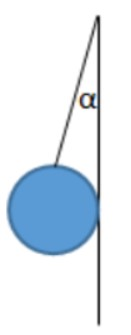
\includegraphics[scale=0.8]{../figs/VN10-2021-PH-TP011-3.jpg}
	\end{center}
}
\loigiai{
	
	Các lực tác dụng lên quả cầu được biểu diễn như hình vẽ:
	\begin{center}
		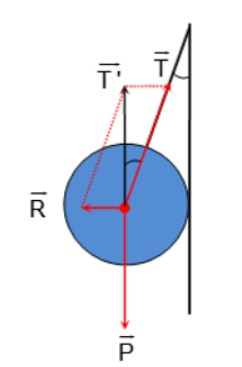
\includegraphics[scale=0.7]{../figs/VN10-2021-PH-TP011-4.jpg}
	\end{center}
	Điều kiện cân bằng của quả cầu là:
	$$\vec{R}+\vec{T}=\vec{T}'=-\vec{P}.$$
	Ta có:
	$$\tan\alpha=\dfrac{R}{P}\Rightarrow R=P\cdot \tan\alpha=\SI{22,6}{\newton}.$$
}
	\item \mkstar{4}

\cauhoi{ Một vật có trọng lượng 60N được treo vào vòng nhẫn nhẹ O (coi là chất điểm). Vòng nhẫn được giữ bằng hai dây nhẹ OA và OB. Biết OA nằm ngang còn OB hợp với phương thẳng đứng góc $45^\circ$ (hình vẽ). Tìm lực căng của dây OA và OB.
	\begin{center}
		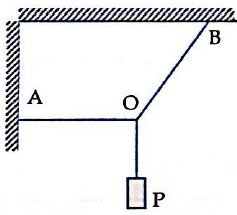
\includegraphics[scale=0.8]{../figs/VN10-2021-PH-TP011-1.jpg}
	\end{center}
}
\loigiai{
	
	\begin{center}
		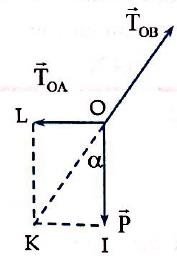
\includegraphics[scale=0.8]{../figs/VN10-2021-PH-TP011-2.jpg}
	\end{center}
	
	Các lực tác dụng vào điểm treo O như hình vẽ.
	
	Góc $\alpha$ là góc giữa OP và OB, $\alpha=45^\circ$.
	$$\text{OI}=\text{OK}\cdot \cos \alpha\Rightarrow \text{OK}=\dfrac{\text{OI}}{\cos \alpha}\Rightarrow T_\text{OB}=\dfrac{P}{\cos \alpha}=60\sqrt{2}\ \text{N} $$.
	
	Tương tự:   $$T_\text{OA}=T_\text{OB}\cdot \sin 45^\circ=60\ \text{N}$$
}
\end{enumerate}